\chapter{Reverberation Mapping Analysis of NGC4593}
\label{cap: Results}

\section{Line Determination}

 The first part of the reverberation mapping analysis is the identification of emission lines in the spectrum of NGC 4593. Figure \ref{fig:AVG_RMS_SPECTRUM} shows her the optical part of the spectrum, while figure \ref{fig:UV_uncalibrated_AVG_RMS} the UV part between 1100 and 1700 $\AA$. \\
 The optical spectrum shows multiple strong broad emission lines. With H$_\alpha$ as the strongest it shows the Balmer lines up to H$_\epsilon$, as well as some Helium lines, like He\,II $\lambda 4685$, He\,I $\lambda 5875$ and He\,I $\lambda 7065$. A significant broad emission line complex can be seen in the far red spectrum with the Oxygen line O\,I $\lambda 8446$ and Ca\,II lines. Especially the O\,I $\lambda 8446$ line is of particular interest in this thesis, as it shows variation and features that could indicate possible bowen fluorescence processes, which was never actively measured before.\\
 The bowen fluorescence of O\,I $\lambda 8446$ is typical driven by the emission of the Ly$_\beta$ line, which lies outside the spectral range of the HST Campaign. However, as can be seen in figure \ref{fig:UV_uncalibrated_AVG_RMS}, Ly$_\alpha$ lies still in the spectral range of the campaign, as the most blue broad line of the taken spectra. 
 
 
\begin{figure}[!htbp]
	\centering
	\makebox[\textwidth][c]{%
		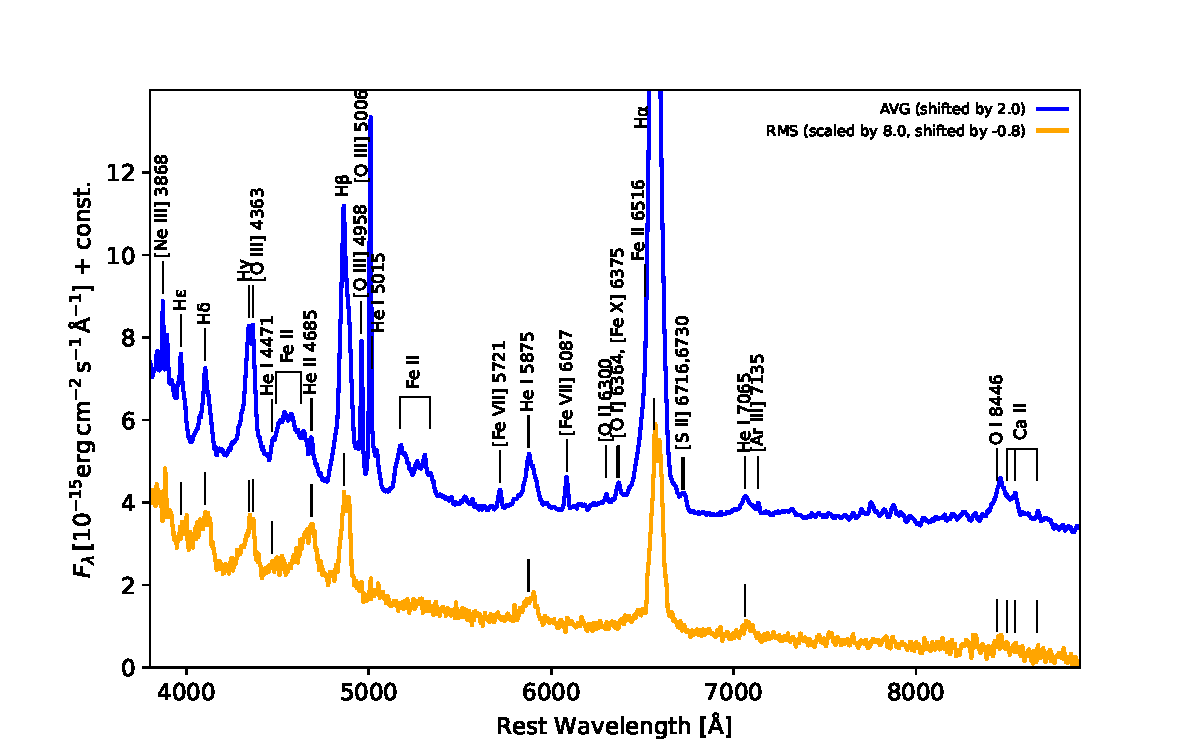
\includegraphics[width=1.1\textwidth]{pictures/Chapter4/avg_rms_spec/avg_rms_spec.pdf}}
	\caption{Optical AVG and RMS spectrum with determined emission lines.}
	\label{fig:AVG_RMS_SPECTRUM}
\end{figure}

\begin{figure}[!htbp]
	\centering
	\makebox[\textwidth][c]{%
		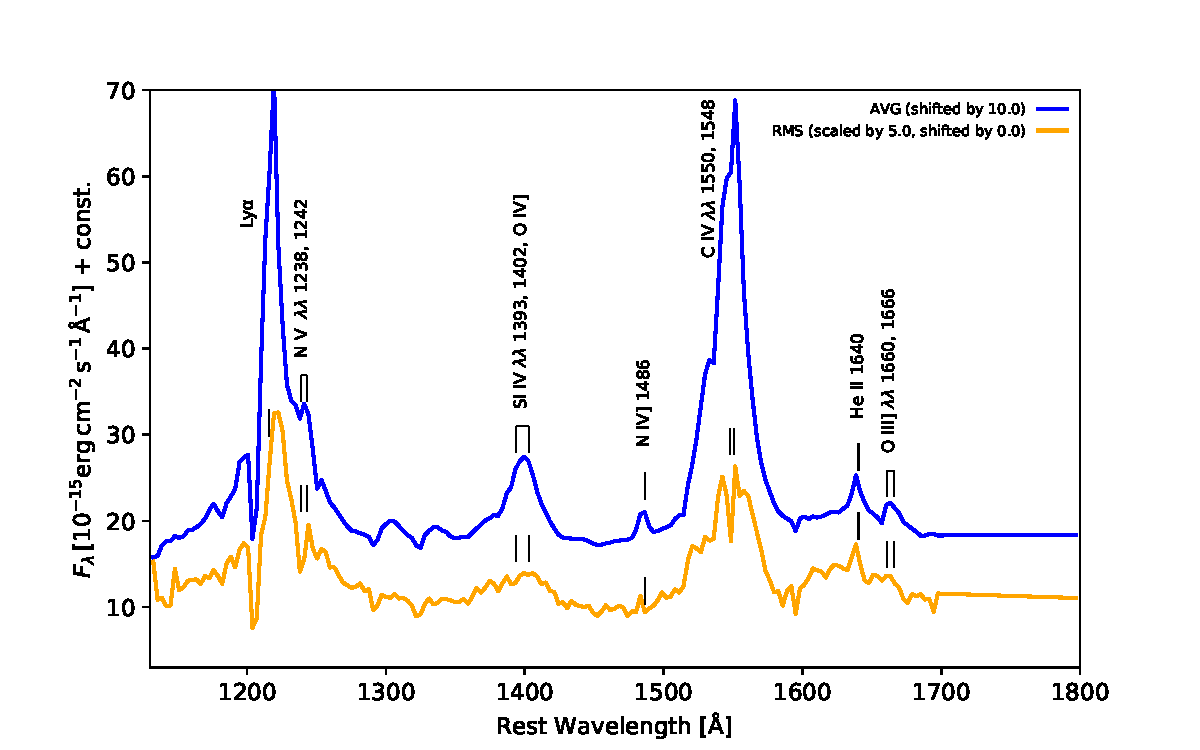
\includegraphics[width=1.1\textwidth]{pictures/Chapter4/avg_rms_spec/UV_uncalibrated_AVG_RMS.pdf}}
	\caption{UV spectrum AVG and RMS spectrum with determined emission lines}
	\label{fig:UV_uncalibrated_AVG_RMS}
\end{figure}


\section{Lightcurves}
...
\subsection{Continua}
...
\begin{figure}[!ht]
	\centering
	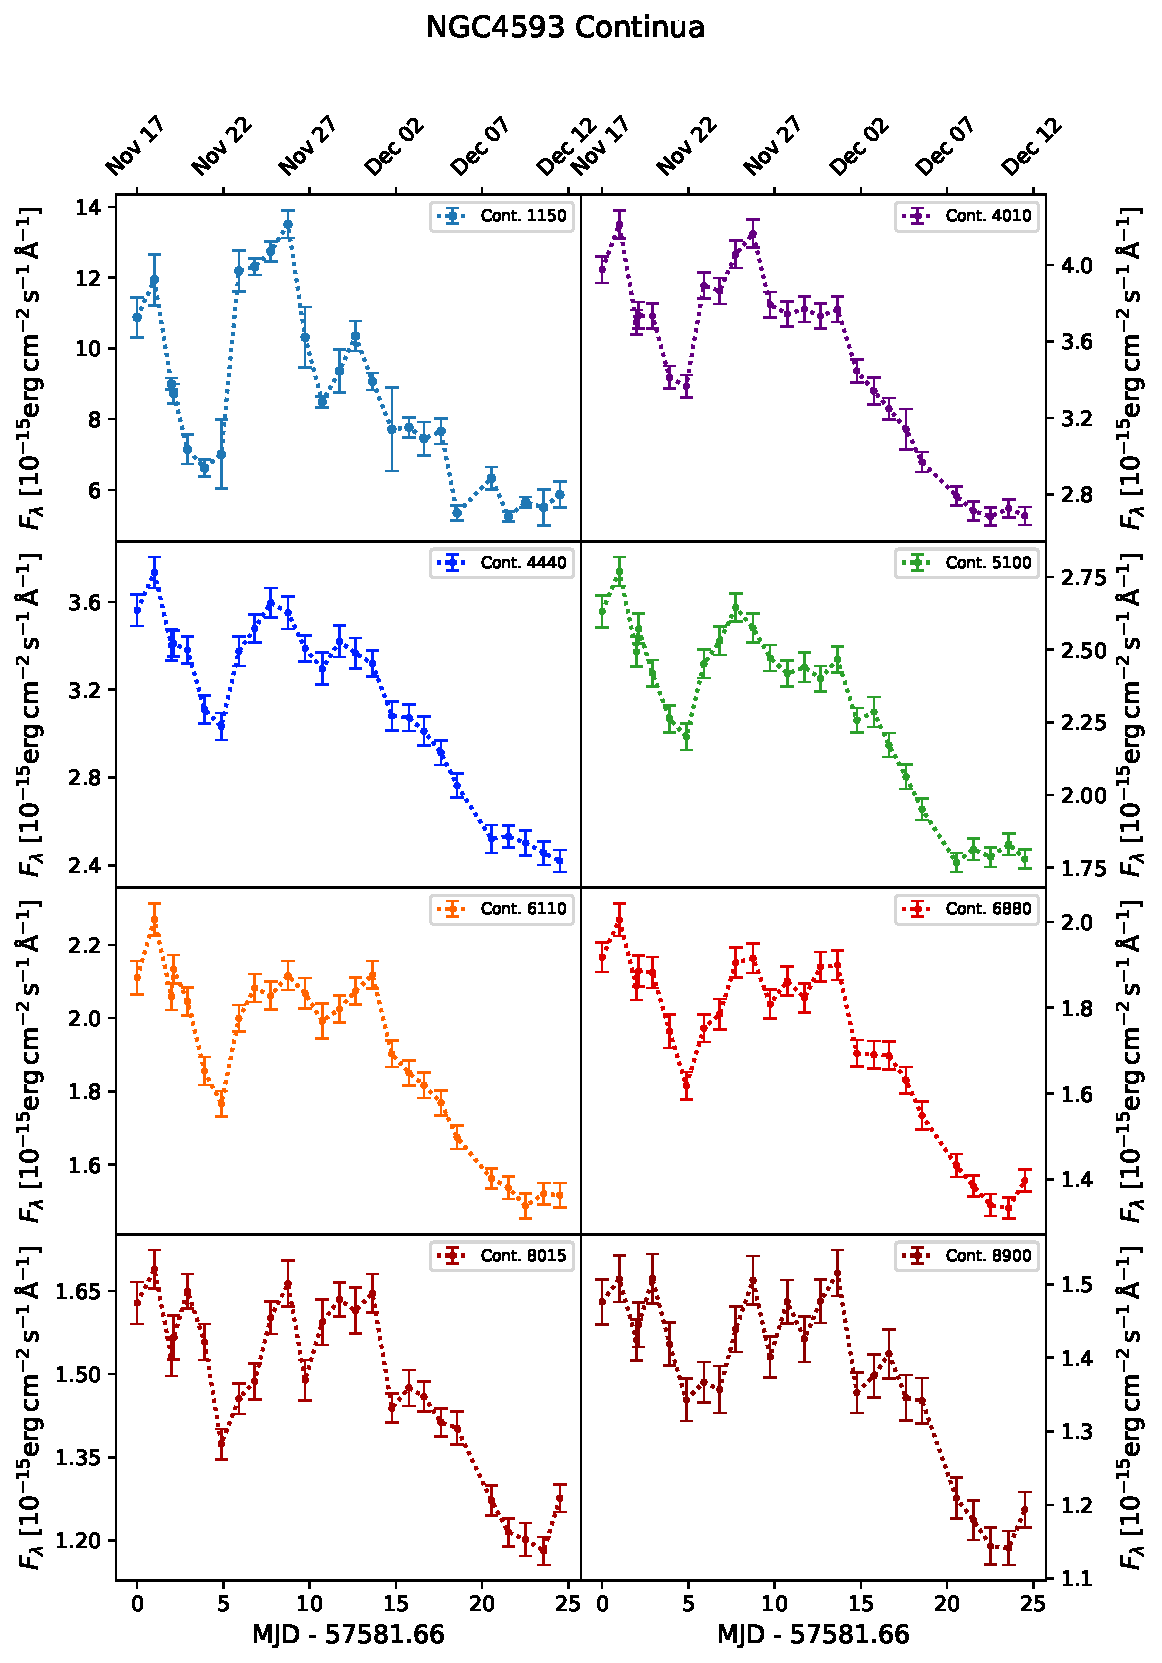
\includegraphics[width=0.9\textwidth]{pictures/Chapter4/lightcurves/NGC4593_Continua.pdf}
	\caption{...}
	\label{fig:continua_lightcurves}
\end{figure}

\subsection{Emission Lines}
...
\begin{figure}[!ht]
	\centering
	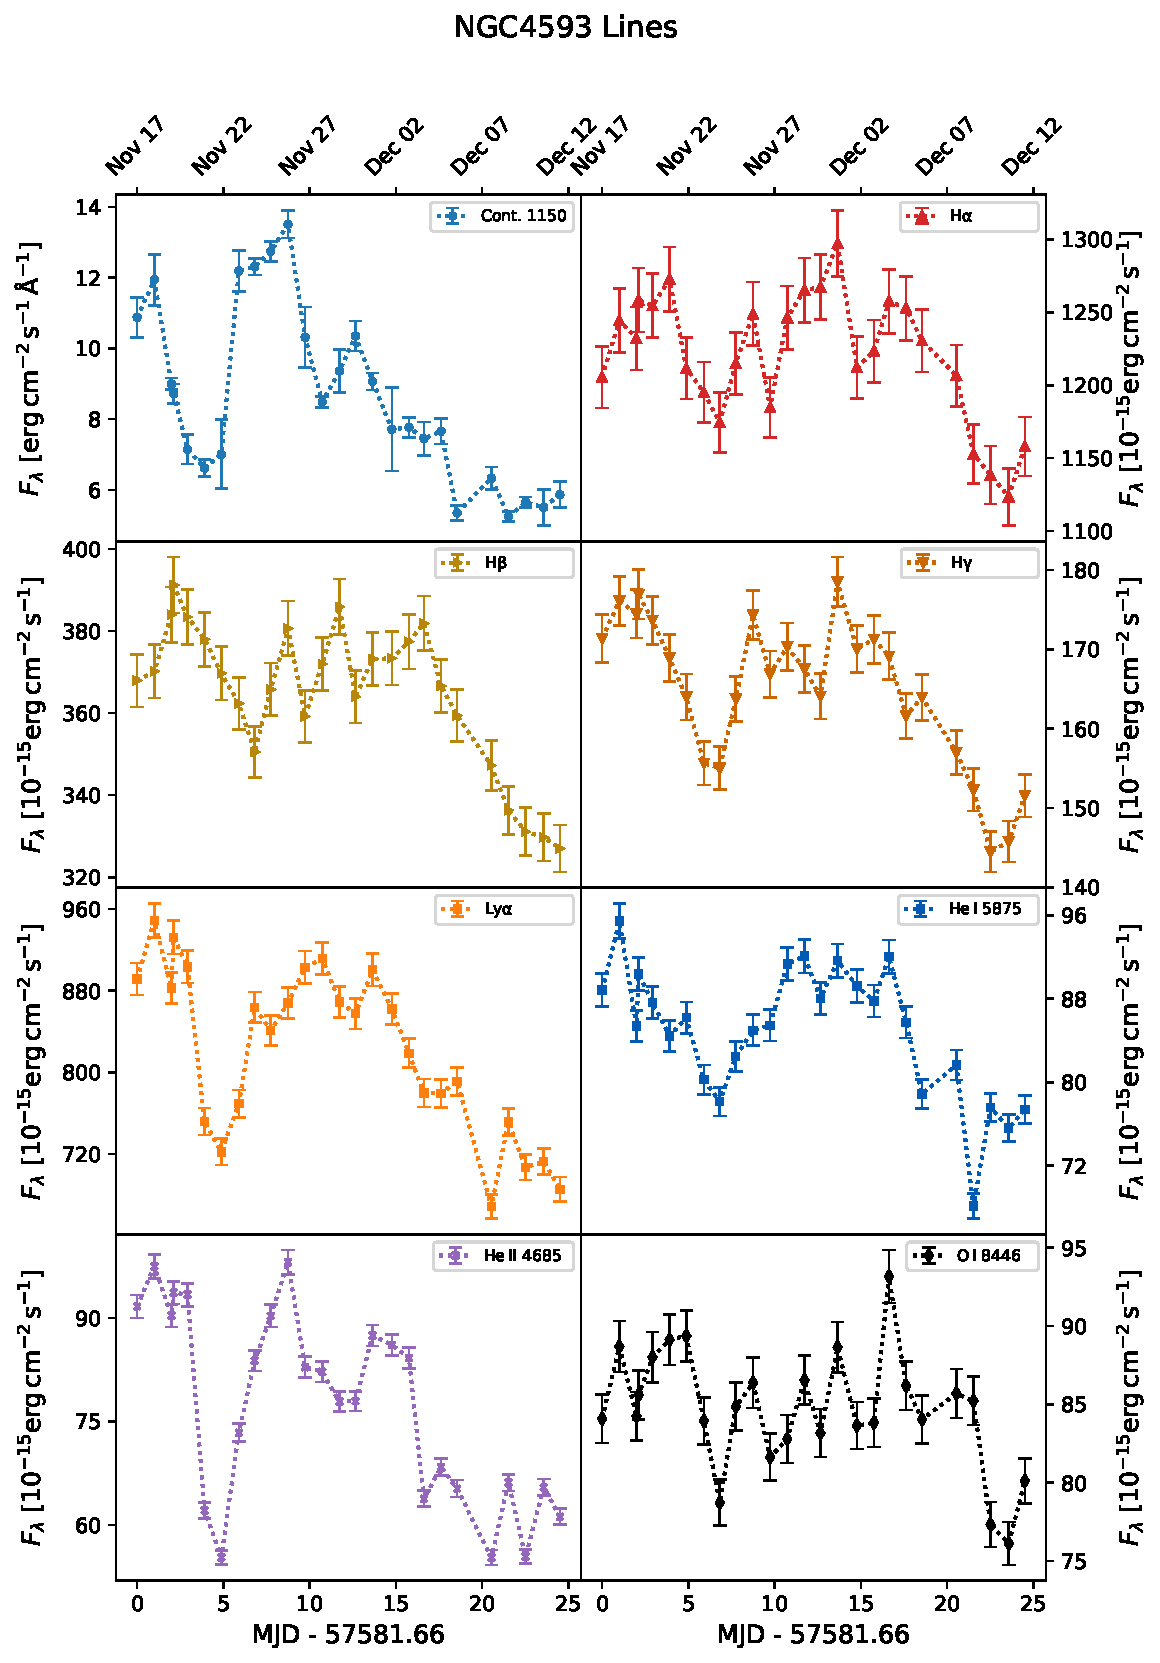
\includegraphics[width=0.9\textwidth]{pictures/Chapter4/lightcurves/NGC4593_Lines.pdf}
	\caption{AVG RMS Spektrum}
	\label{fig:emission_line_lightcurves}
\end{figure}

\section{Line Profiles}

\begin{figure}[!ht]
	\centering
	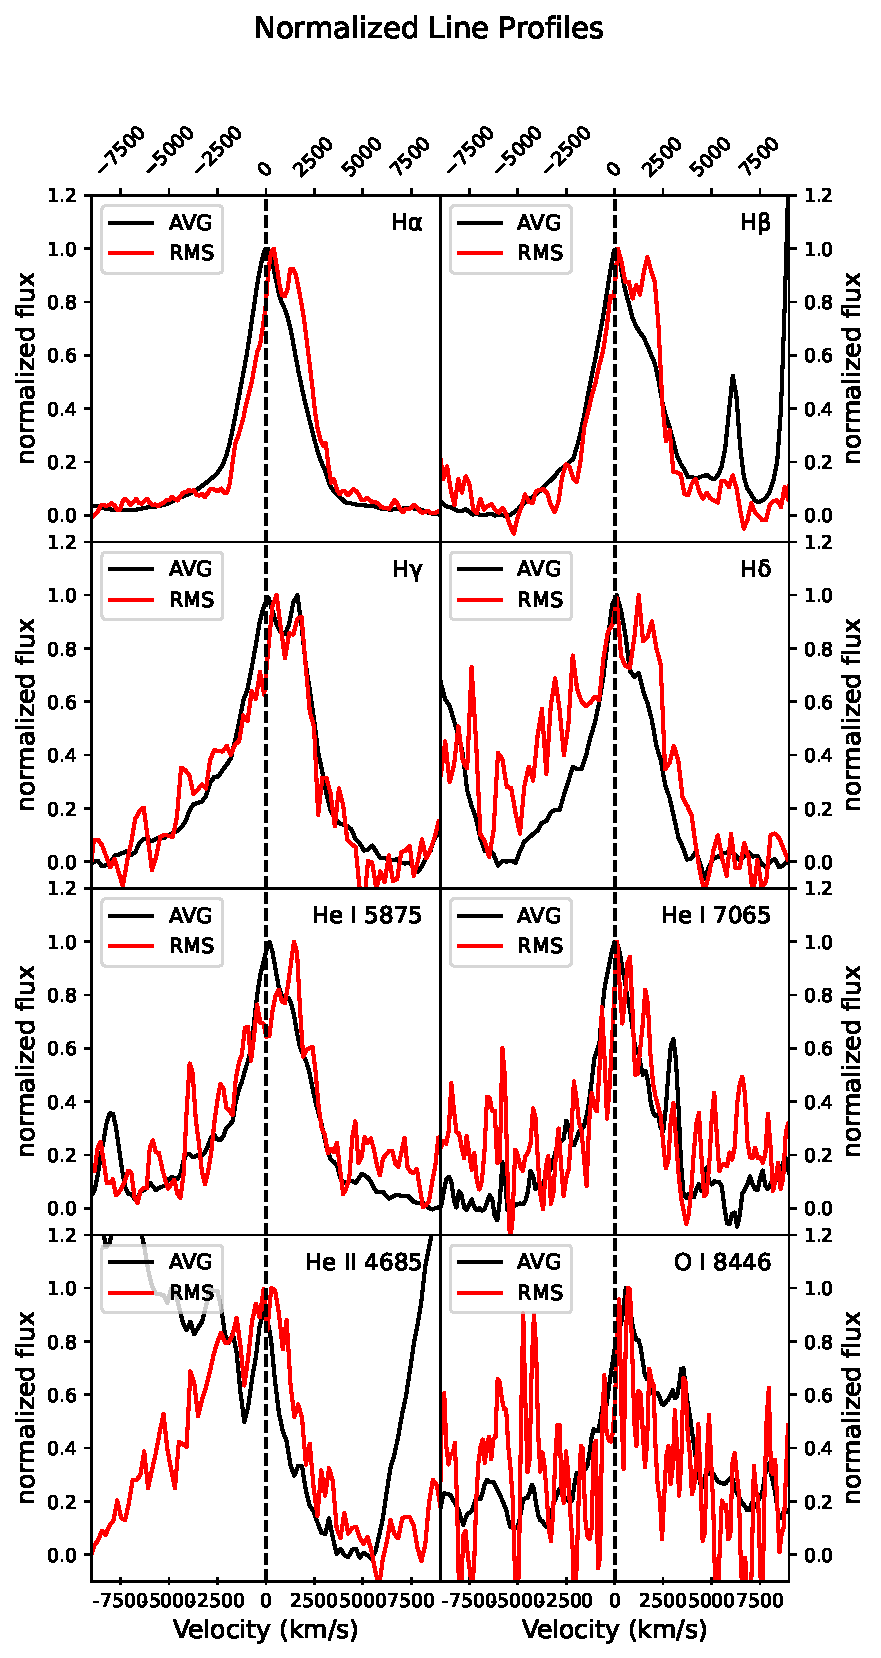
\includegraphics[width=0.8\textwidth]{pictures/Chapter4/line_profiles/Normalized_Line_Profiles.pdf}
	\caption{AVG RMS Spektrum}
	\label{fig:line_profiles}
\end{figure}

\section{Time Lag and BH Masses}

\begin{figure}[!ht]
	\centering
	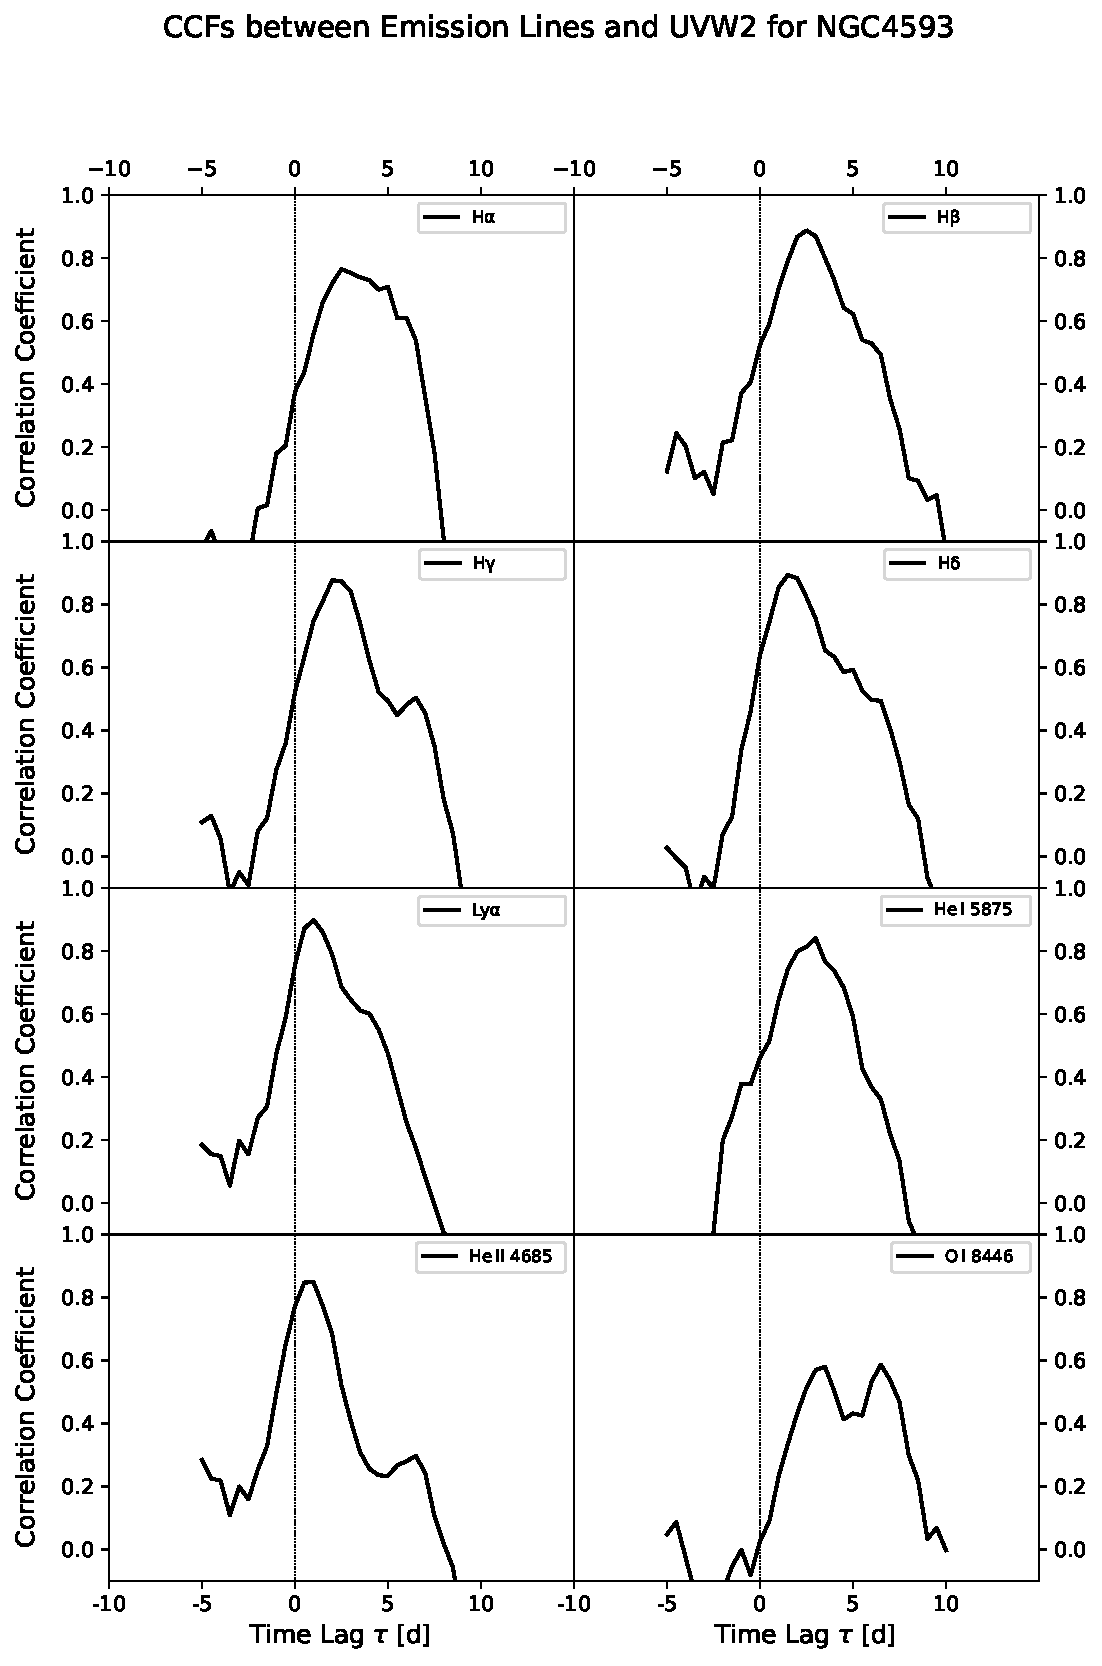
\includegraphics[width=0.9\textwidth]{pictures/Chapter4/ccfs/CCFs_H_He_LyA_O_UVW2.pdf}
	\caption{AVG RMS Spektrum}
	\label{fig:ccfs}
\end{figure}

\begin{figure}[!ht]
	\centering
	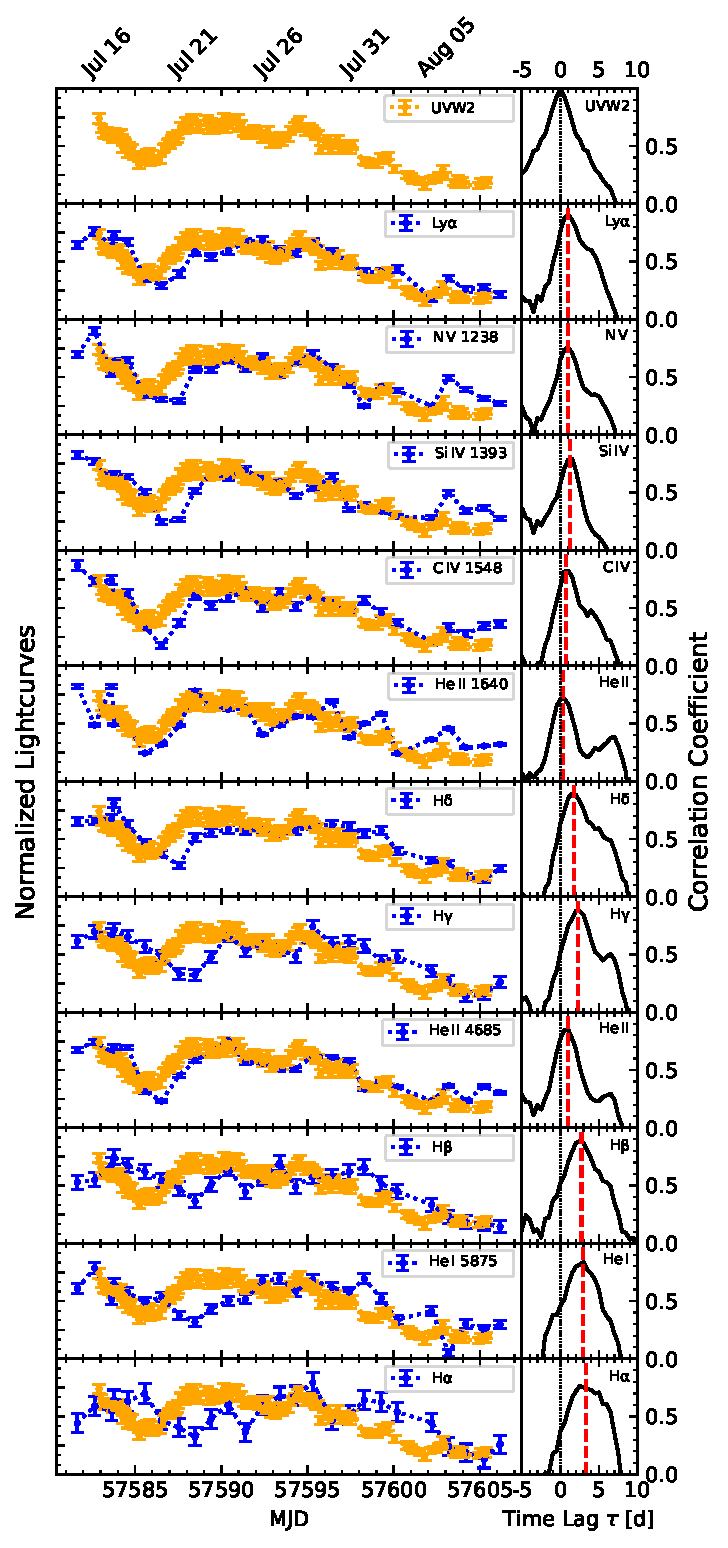
\includegraphics[width=0.7\textwidth]{pictures/Chapter4/lighcurves_and_ccfs_and_time_lag_tables/UV_to_HAlpha_ccfs_and_reference_lightcurves.pdf}
	\caption{AVG RMS Spektrum}
	\label{fig:ccfs_lightcurves}
\end{figure}

\section{Bowen Fluorescence}